\documentclass[../main]{subfiles}

\begin{document}
\section{Fundamento teórico}

\subsection{Hardware}

\subsubsection{Microcontrolador}

ESP32 es una familia de microcontroladores que pertenece a Espressif
caracterizada por su variedad de módulos integrados orientados a
telecomunicaciones por Bluetooth y Wi-Fi. \supercite{ESP32_espressif}

La serie ESP32-DevKitC, en particular, es notable por tener una abundancia de
pines expuestos para facilitar su conexión y uso.
El presente prototipo utiliza un microcontrolador ESP32-DevKitC V4, mismo que
tiene integrados un botón de reinicio, así como un puerto Micro-USB
conectado a un puente USB-a-UART \supercite{devkitv4}.
Una imagen del microcontrolador con detalles anotados es provista en la figura
\ref{esp32devkitcv4image}.

Entre sus componentes, son de interés un módulo ESP32-WROOM-32 integrado con un
microprocesador ESP-D0WDQ6, una interfaz serial de periféricos con
\qty{4}{\mega\byte} de memoria flash integrada, una antena y un oscilador de
cristal con frecuencia \qty{40}{\MHz}, \supercite{esp32wroom32doc}
tal como se puede observar en la figura \ref{esp32wroom32esq}.

\begin{figure}[H]
	\centering
	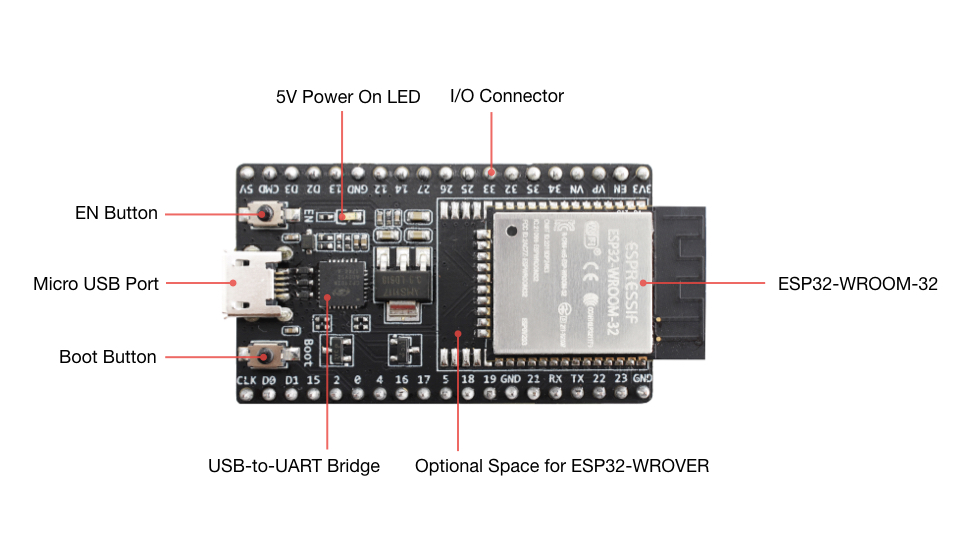
\includegraphics[width=0.95\textwidth]{res/esp32-devkitc-v4-functional-overview.jpg}
	\caption{Descripción del ESP32-DevKitC V4 \supercite{devkitv4}}
	\label{esp32devkitcv4image}
\end{figure}

\begin{table}[H]
	\centering
	\begin{tabularx}{0.9\textwidth}{l X}
		\toprule
		\multicolumn{1}{c}{\textbf{ Componente }} &
		\multicolumn{1}{c}{\textbf{ Descripción }}                                                                                                                                                                \\
		\midrule
		ESP32-WROOM-32                            & Módulo con el ESP32.                                                                                                                                          \\
		EN                                        & Botón de reinicio.                                                                                                                                            \\
		Boot                                      & Botón de descarga. Mantenerlo presionado y luego presionar \textit{EN} inicia el \textit{Modo de descarga de firmware}, que opera a través del puerto serial. \\
		USB-to-UART Bridge                        & Un chip de puente USB-UART. Provee velocidades de transferencia de hasta \qty{3}{\mega\byte\per\s}.                                                           \\
		Micro USB Port                            & Interfaz USB. Provee energía a la placa y puede comunicar a una computadora con el módulo ESP32-WROOM-32.                                                     \\
		5V Power On LED                           & Se enciende cuando está conectado a la placa un suministro de energía de \qty{5}{\V} externo o por USB.                                                       \\
		I/O                                       & La mayoría de los pines del módulo ESP están conectados con los que sobresalen de la placa. Pueden poseer funcionalidad I2C, SPI, etc.                        \\
		\bottomrule
	\end{tabularx}
	\caption{ESP32-DevKitC V4 con el módulo ESP32-WROOM-32 \supercite{devkitv4}}
	\label{esp32devkitcv4_descrp}
\end{table}

\begin{landscape}
	\begin{figure}[H]
		\centering
		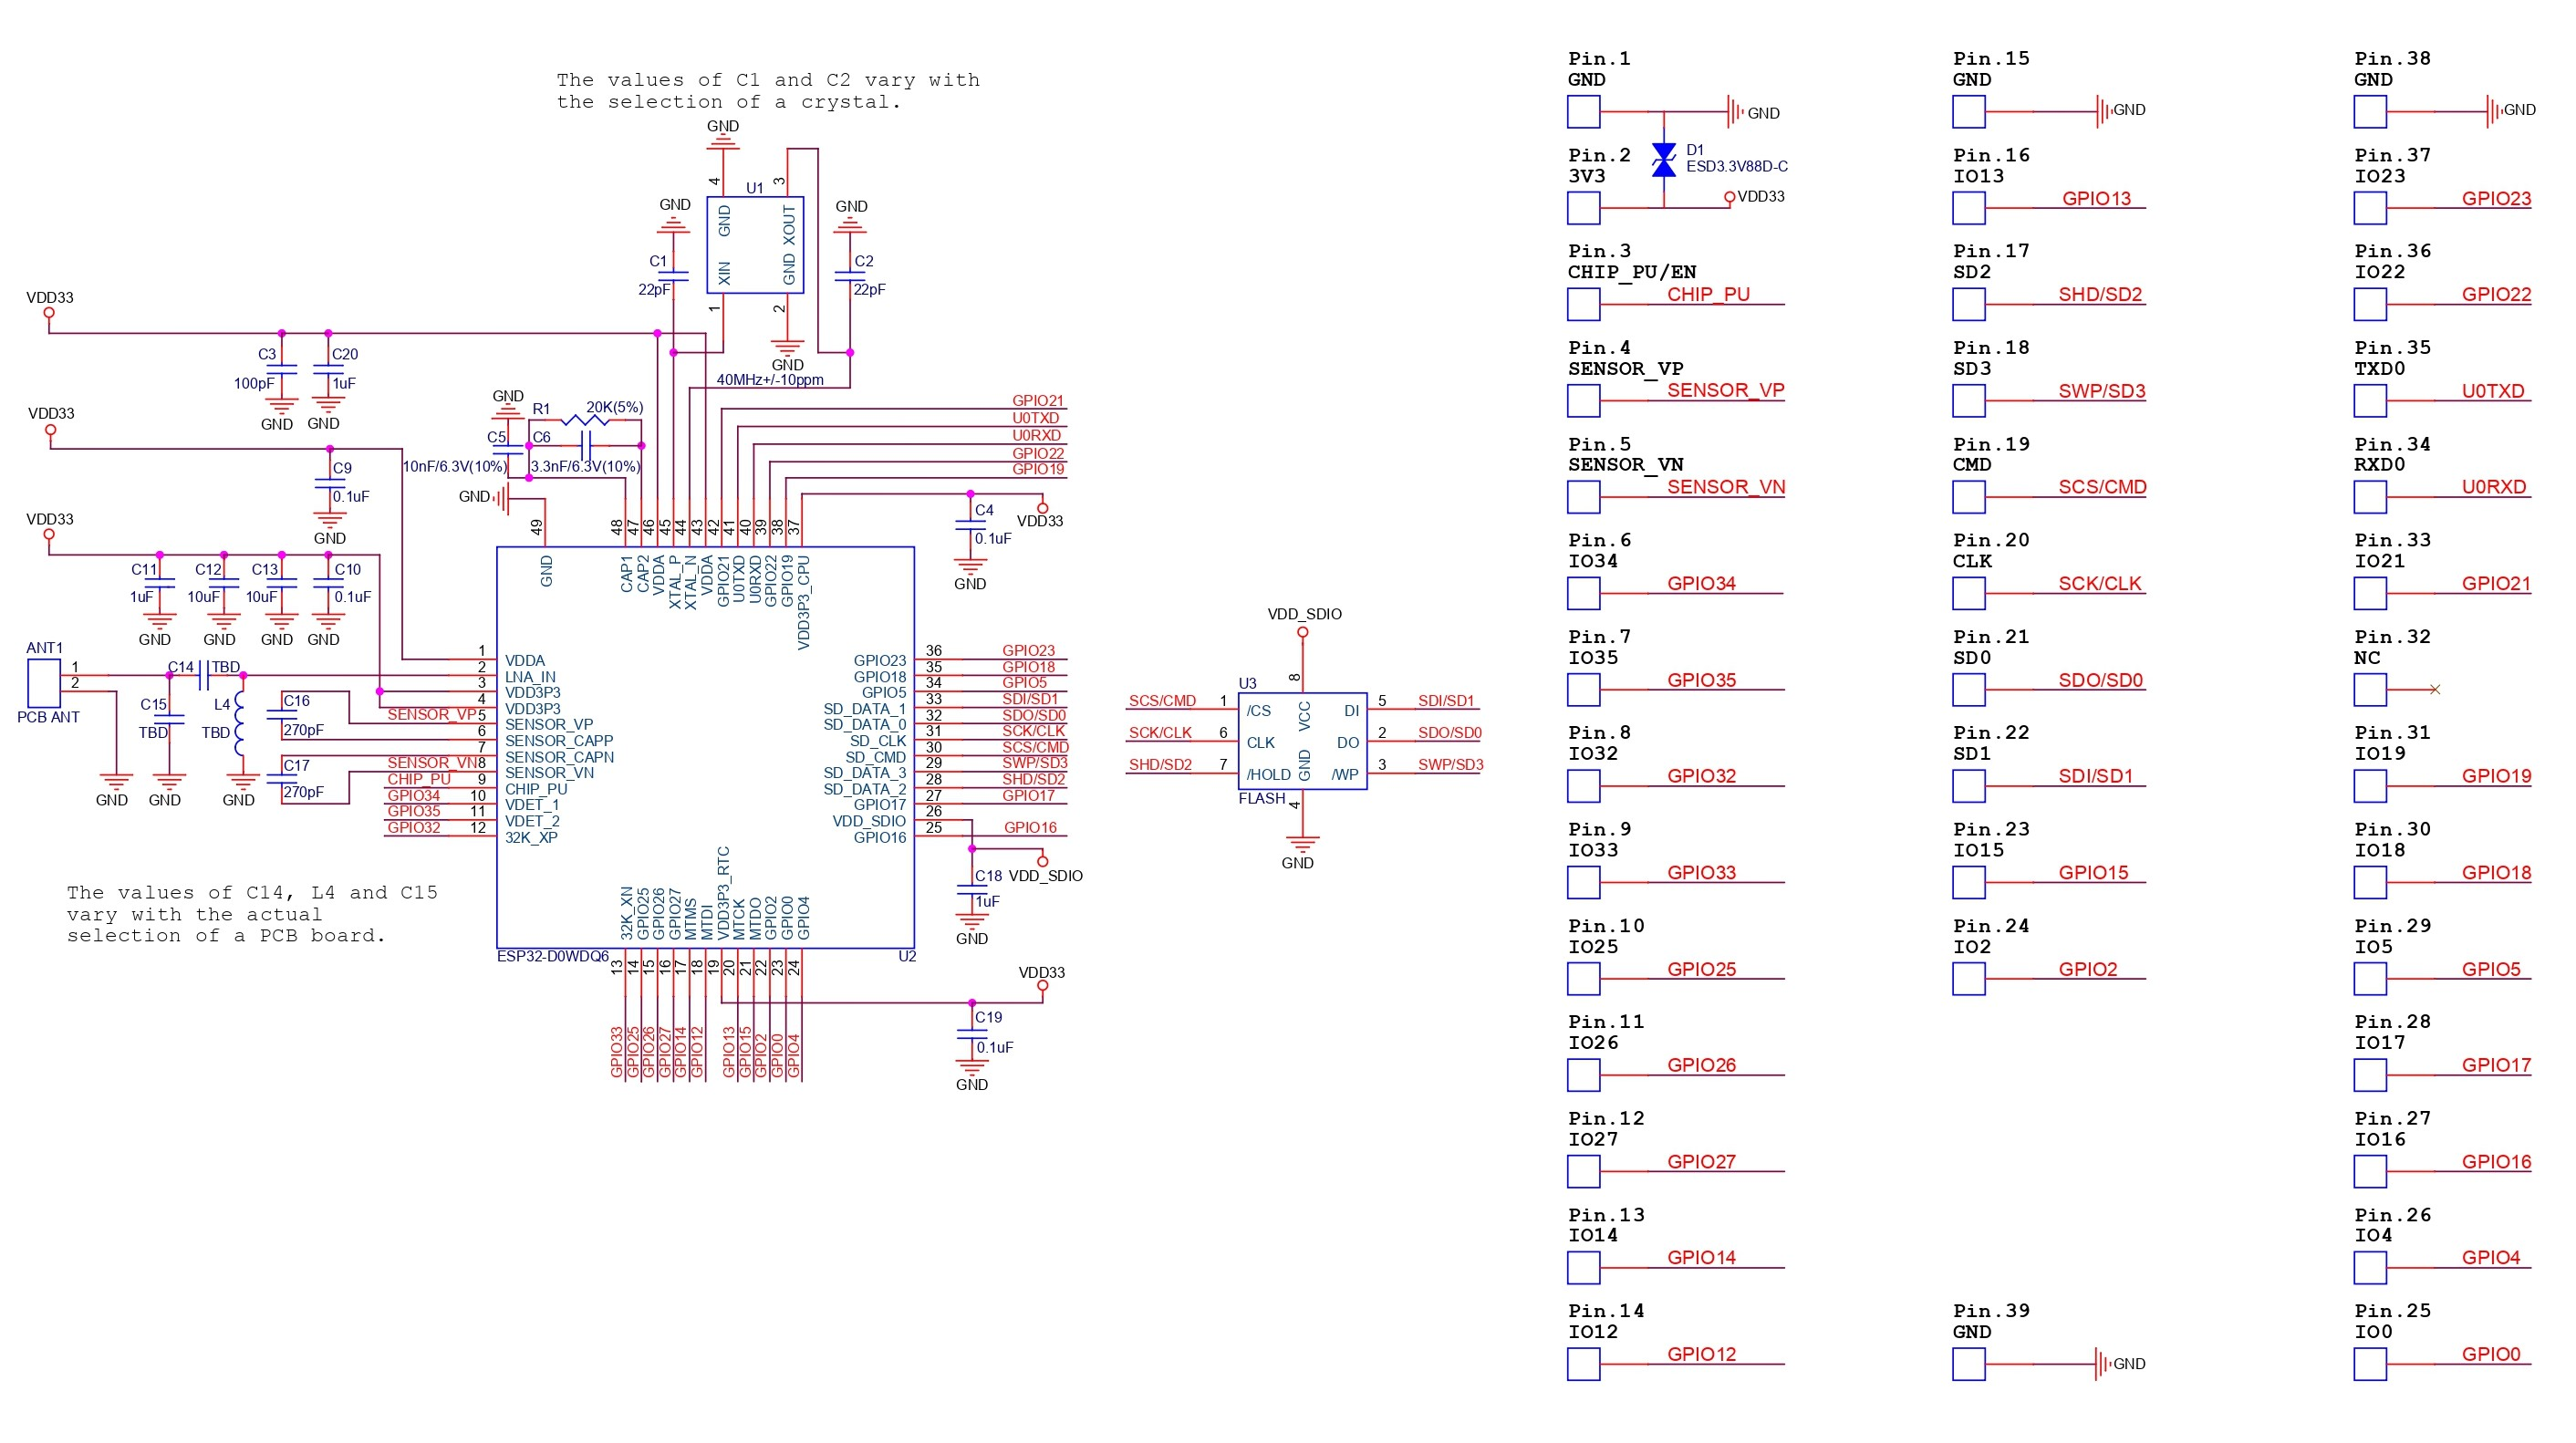
\includegraphics[height=0.85\textheight]{res/esp32-wroom-32_diagram.jpg}
		\caption{Esquema del ESP32-WROOM-32 \supercite{esp32wroom32doc}}
		\label{esp32wroom32esq}
	\end{figure}
\end{landscape}

\begin{figure}[H]
	\centering
	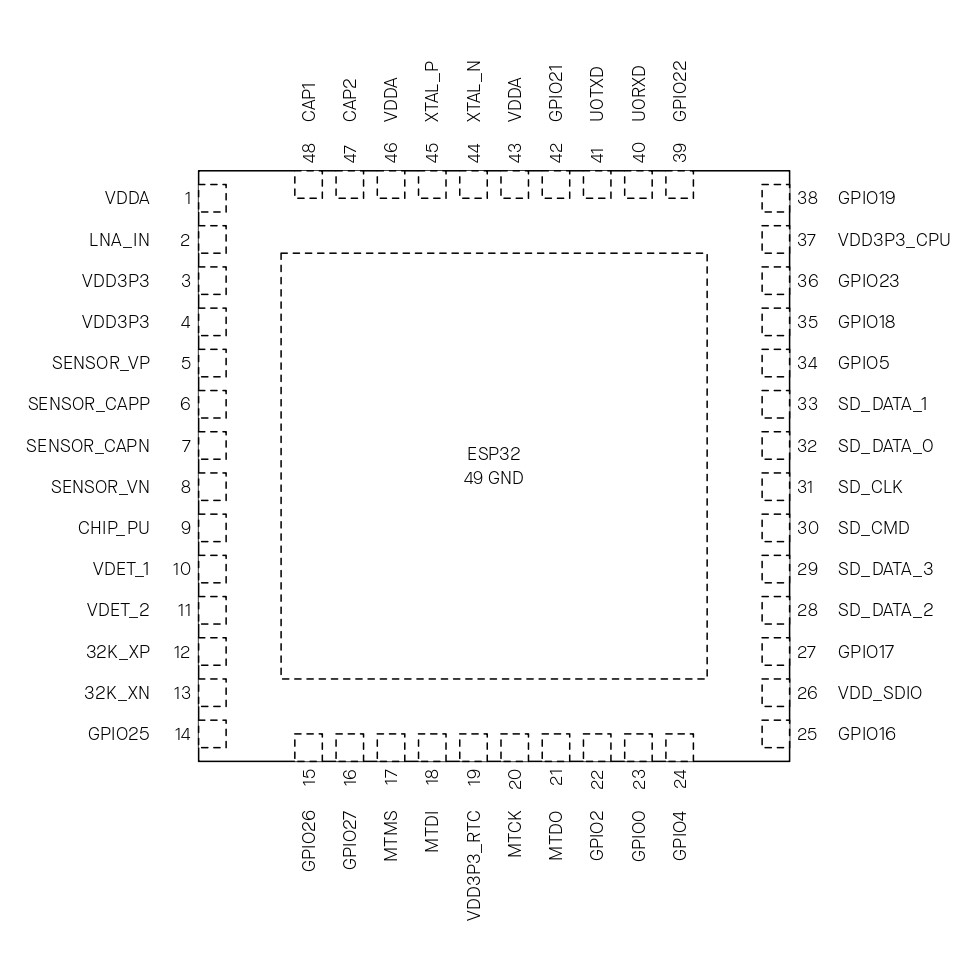
\includegraphics[width=\textwidth]{res/esp32_datasheet_en_page-0013.jpg}
	\caption{Diagrama de pines del ESP32-D0WDQ6 \supercite{esp32d0wdq62doc}}
	\label{fig:esp32d0wdq62pines}
\end{figure}

\subsubsection{Sensor BME280}

El sensor BOSCH-BME280 es capaz de medir humedad relativa, presión
barométrica y temperatura ambiente. \supercite{boschbme280descr}
Algunas características se encuentran en la tabla \ref{tab:bme280techdata}.

\begin{figure}[H]
	\centering
	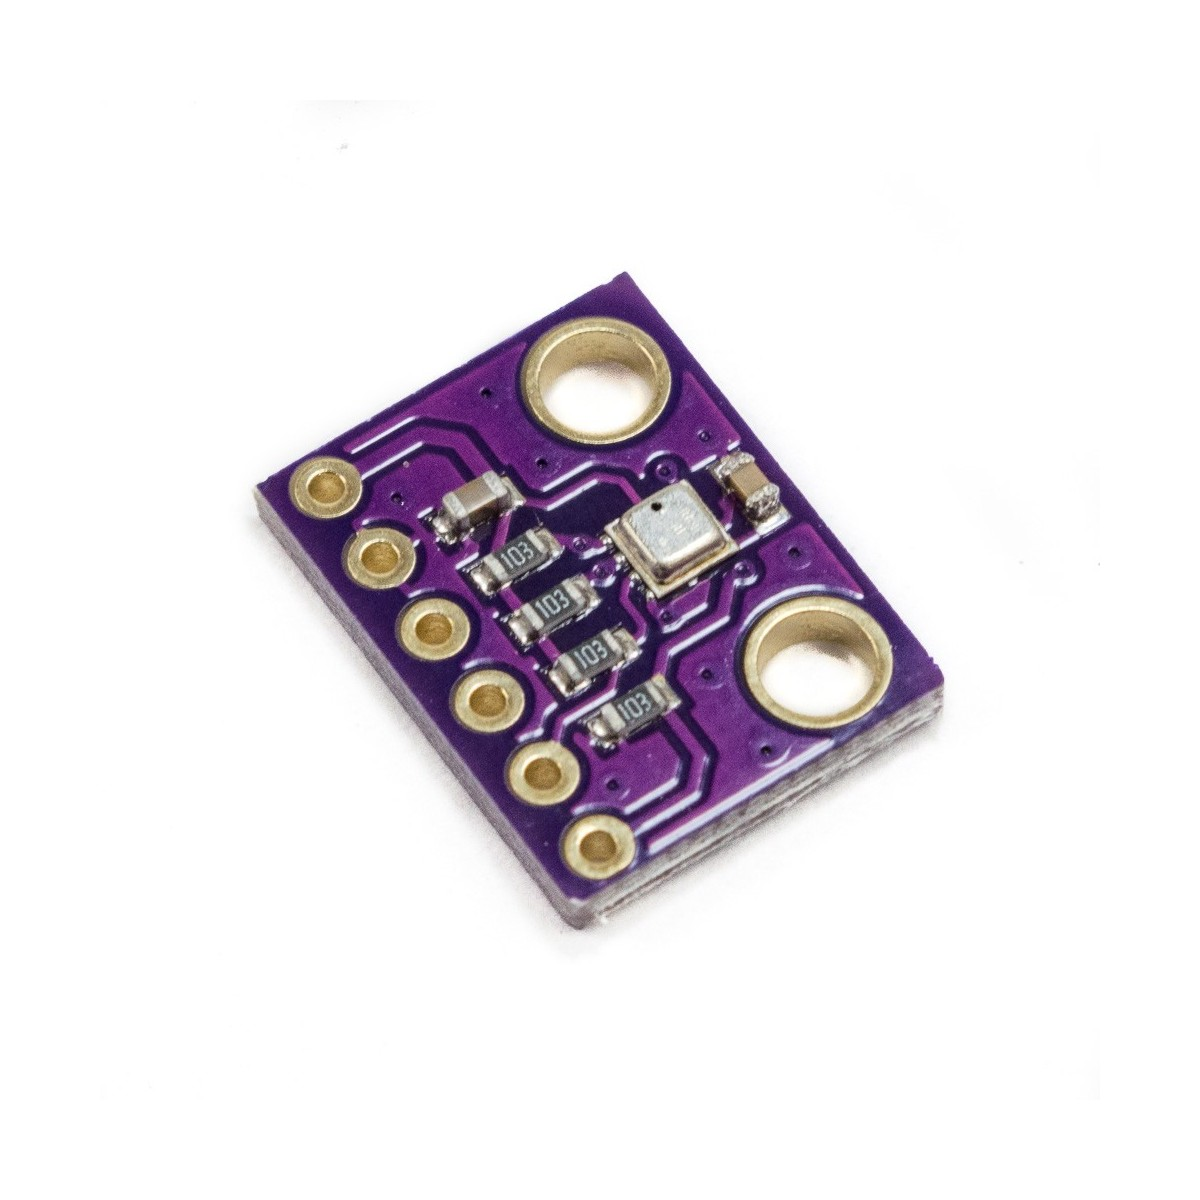
\includegraphics[height=6cm]{res/sensor-bme280-presion-temperatura-y-humedad.jpg}
	\caption{Sensor BME280 \supercite{bme280image}}
	\label{fig:bme280fig}
\end{figure}

\begin{table}[H]
	\centering
	\begin{tabularx}{0.9\textwidth}{l X}
		\toprule
		Rango de operación                       & Presión: \qtyrange{300}{1100}{\hecto\Pa}                           \\
		                                         & Temperatura: \qtyrange{-40}{85}{\degreeCelsius}                    \\
		\midrule
		Voltaje de entrada V\textsubscript{DD}   & \qtyrange{1.71}{3.6}{\V}                                           \\
		Voltaje de entrada V\textsubscript{DDIO} & \qtyrange{1.2}{3.6}{\V}                                            \\
		\midrule
		Interfaz                                 & I\textsuperscript{2}C y SPI                                        \\
		\midrule
		Consumo de corriente                     & \qty{1.8}{\micro\A} @ \qty{1}{\Hz} (humedad, temperatura)          \\
		                                         & \qty{2.8}{\micro\A} @ \qty{1}{\Hz} (presión, temperatura)          \\
		                                         & \qty{3.6}{\micro\A} @ \qty{1}{\Hz} (humedad, presión, temperatura) \\
		                                         & \qty{0.1}{\micro\A} (inactivo)                                     \\
		\midrule
		\textbf{Sensor de humedad}               &                                                                    \\
		Tiempo de respuesta                      & \qty{1}{\s}                                                        \\
		Tolerancia de precisión                  & \qty[parse-numbers=false]{\pm\ 3}{\percent} humedad relativa       \\
		Histéresis                               & \qty[parse-numbers=false]{\leq 2}{\percent} humedad relativa       \\
		\midrule
		\textbf{Sensor de presión}               &                                                                    \\
		Ruido RMS                                & \qty{0.2}{\Pa}                                                     \\
		Error de sensitividad                    & \qty[parse-numbers=false]{\pm\ 0.25}{\percent}                     \\
		Coeficiente de temperatura ajustado      & \qty[parse-numbers=false,per-mode=fraction]{\pm\ 1.5}{\Pa\per\K}   \\
		\midrule
		Base                                     & LGA de 8 pines con tapa de metal                                   \\
		Dimensiones                              & \qtyproduct{ 2.5 x 2.5 x 0.93 }{\mm\cubed}                         \\
		\bottomrule
	\end{tabularx}
	\caption{Información técnica del BME280 \supercite{boschbme280techdata}}
	\label{tab:bme280techdata}
\end{table}

\subsubsection{Sensor MQ135}

El sensor MQ135 mide la calidad del aire utilizando \ce{SnO2}, cuya
conductividad varía cuando entra en contacto con impurezas en el aire.
\supercite{mq135winson}
En la tabla \ref{tab:mq135conditions} son mencionadas algunas características
del sensor.

\begin{figure}[H]
	\centering
	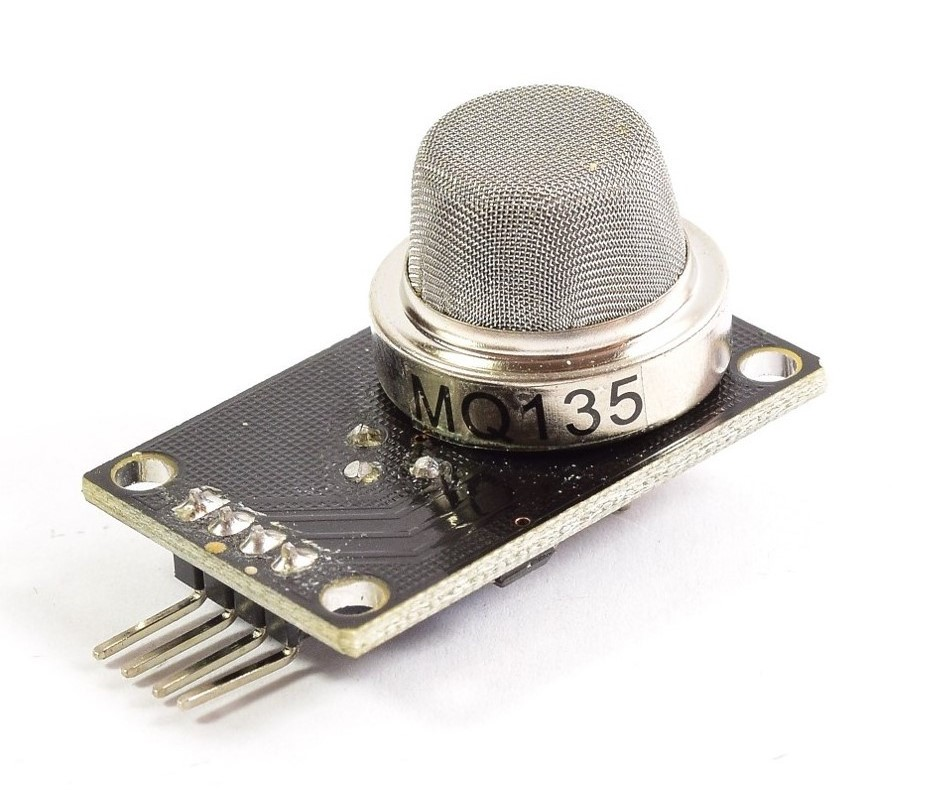
\includegraphics[scale=0.5]{res/sensor-mq-135-gas-calidad-aire.jpg}
	\caption{Sensor MQ-135 \supercite{mq135image}}
	\label{fig:mq135fig}
\end{figure}

\begin{table}[H]
	\centering
	\begin{tabular}{m{6cm} m{6cm}}
		\toprule
		Parámetro                                      & Condición                                                                                      \\
		\midrule
		\textbf{Condiciones de trabajo}                &                                                                                                \\
		Voltaje en circuito                            & \qty{5.0(1)}{\V} AC o DC                                                                       \\
		Voltaje de calentamiento                       & \qty{5.0(1)}{\V} AC o DC                                                                       \\
		Resistencia de calentador                      & 33 $\Omega\ \pm$ 5\%                                                                           \\
		\midrule
		\textbf{Condiciones de ambiente}               &                                                                                                \\
		Temperatura de uso                             & \qtyrange{-10}{45}{\degreeCelsius}                                                             \\
		Humedad relativa permitida                     & \qty[parse-numbers=false]{< 95}{\percent}                                                      \\
		Valores de concentración de oxígeno permitidos & \qty{21}{\percent} en condiciones normales, mínimo de \qty[parse-numbers=false]{> 2}{\percent} \\
		\bottomrule
	\end{tabular}
	\caption{Condiciones de trabajo normales y de ambiente permitidos del MQ-135 \supercite{mq135hanwei}}
	\label{tab:mq135conditions}
\end{table}

\subsubsection{Sensor ECH2O EC-5}

El sensor EC-5 mide la humedad del suelo mediante la resistencia entre dos
electrodos, la cual varía con proporcionalidad inversa respecto a la humedad
del suelo cuando el sensor está inserto en él.
\supercite{ec5humedadsuelosensor}
Algunas especificaciones pueden encontrarse en la tabla \ref{tab:ec5tecesp}

\begin{figure}[H]
	\centering
	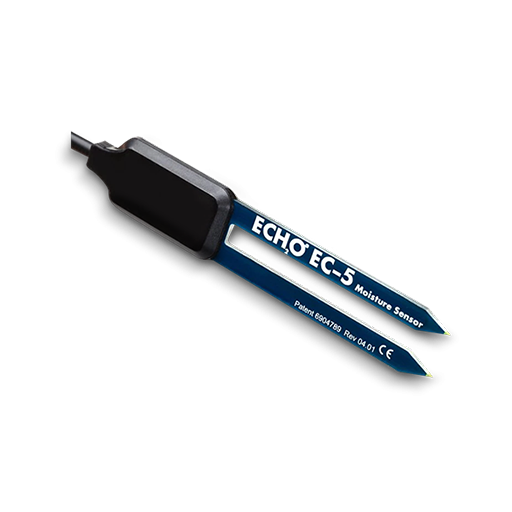
\includegraphics[scale = 0.6]{res/sonde-ec-5-decagon_.png}
	\caption{Sensor Decagon EC-5 \supercite{ec5image}}
	\label{fig:ec5fig}
\end{figure}

\begin{table}[H]
	\centering
	\begin{tabular}{c c}
		\toprule
		\multicolumn{1}{c}{\textbf{ Parámetro }} &
		\multicolumn{1}{c}{\textbf{ Valor }}                                                                 \\
		\midrule
		Tiempo de medición                       & \qty{10}{\ms}                                             \\
		Precisión                                & \qty[parse-numbers=false]{\pm 2}{\percent}                \\
		Requisitos de energía                    & \qtyrange{2.5}{3.6}{\V\textsubscript{DC}} @ \qty{10}{\mA} \\
		Rango de temperaturas                    & \qtyrange{-40}{60}{\degreeCelsius}                        \\
		Rango de medición                        & De 0 hasta saturarse                                      \\
		\bottomrule
	\end{tabular}
	\caption{Especificaciones técnicas del ECH2O EC-5 \supercite{ec5humedadsuelosensor}}
	\label{tab:ec5tecesp}
\end{table}

\subsection{Software}

\subsubsection{Kotlin}

Kotlin es un lenguaje de programación desarrollado por JetBrains que tiene
soporte oficial de Google para desarrollo de aplicativos en Android.
Por defecto es ejecutado en la Máquina Virtual de Java, por lo que la
interoperabilidad Kotlin-Java es alta. \supercite{JetBrains}

Kotlin es considerado estable y moderno en comparación con Java, un lenguaje
conocido por complicaciones de retrocompatibilidad, por lo que es una opción
preferible para desarrollar aplicativos en la plataforma Android.
\supercite{Moskala_Wojda_2017b}

\subsubsection{Android Studio}

Android Studio es el entorno de desarrollo integrado oficial utilizado en el
desarrollo de aplicativos para Android.
Su calidad tiene relación con los componentes que comparte con el ampliamente
reconocido editor IntelliJ IDEA, también desarrollado por JetBrains.
Entre sus herramientas más críticas, destaca el acceso a servicios y
herramientas que provee Google. \supercite{android_developers}

\begin{figure}[H]
	\centering
	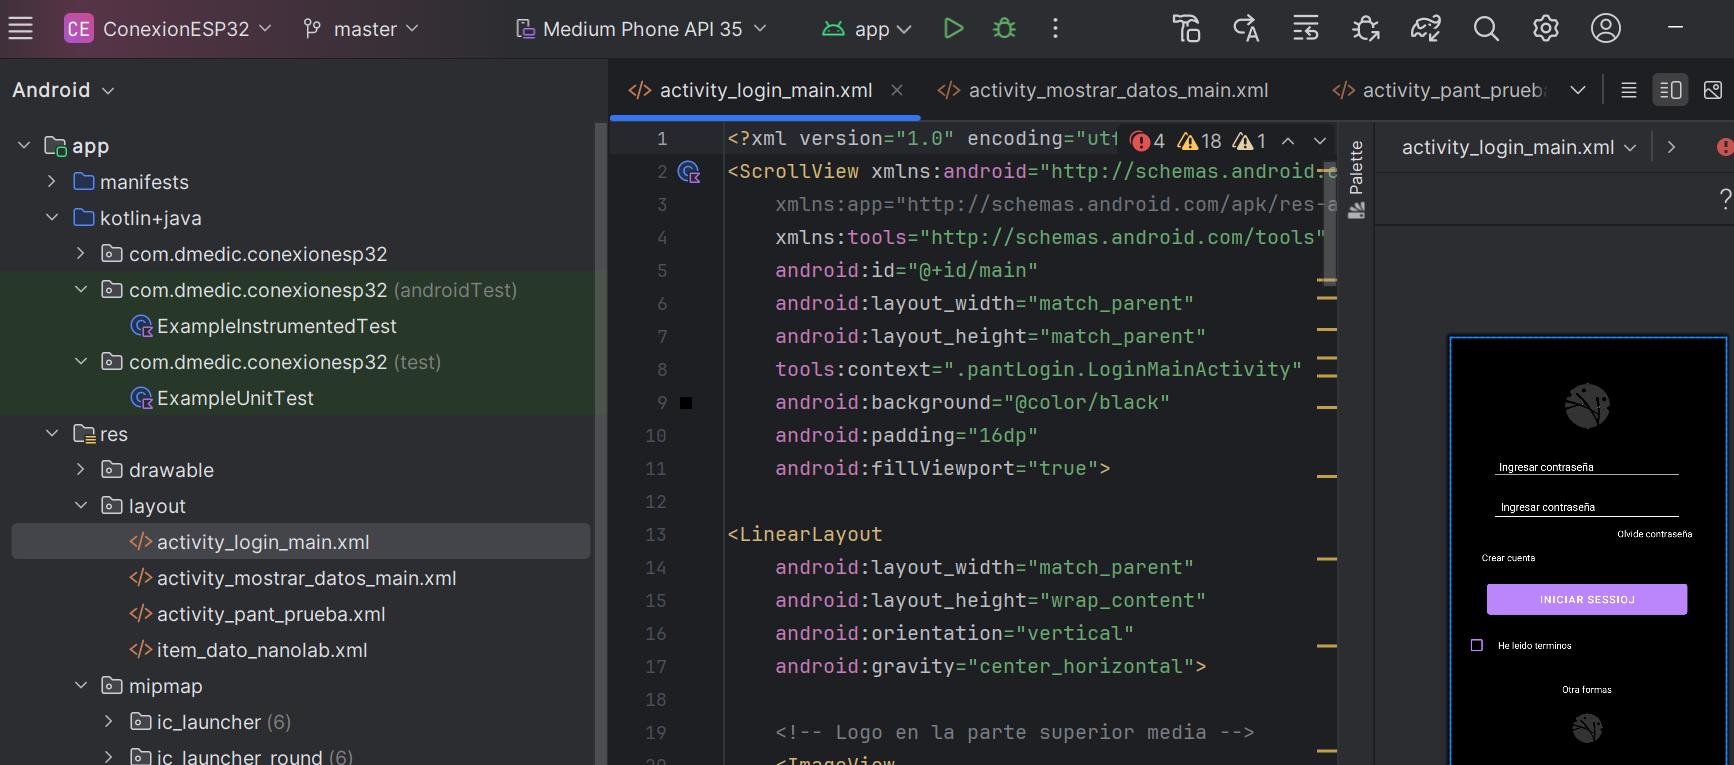
\includegraphics[width=15cm]{res/EjemploDeProgramaAndroidStudio.png}
	\caption{Ejemplo de programa en Android Studio}
	\label{ImagenEjemploAndroidStudio}
\end{figure}
\end{document}
